\section{Discussion and Conclusions}
	As per current literature on spectral fitting of \source, Bearda et al. (2002) and Motch et al. (2002) had arrived at the conclusion that its spectra cannot be reproduced by NLTE model atmospheres \cite{beardaChandra2002AA,motchXmmNewton2002AA}. Earlier, Hartmann et al. (1999) had applied non-local thermodynamic equilibrium (NLTE) models, which included metal line opacities, to the spectrum extracted from the observations by BeppoSAX LECS of \source\ on 25--26 January 1997 \cite{hartmann1999constraining}, where the best fit was using a model consisting of two spectral components. But nevertheless, they obtained a reduced $\chi^2>2$. In the absence of a proper model describing the emission spectrum, it becomes impossible to
derive fundamental parameters such as temperature, neutral hydrogen column density and luminosity \cite{motchXmmNewton2002AA}. Hence, obtaining an acceptable fit for RX J0925 spectrum assumes crucial importance at this juncture.
%	\begin{itemize}
%		\item To include a detailed description of the physics behind the best fit model
%		\item To refer to the original publications containing the XSPEC model components where the physics is described
%		\begin{itemize}
%			\item For \texttt{TBabs}: Wilms et al. \url{https://iopscience.iop.org/article/10.1086/317016/pdf}
%			
%			Now \texttt{phabs}
%			\item For \texttt{ismabs}: Gatuzz et al. \url{https://iopscience.iop.org/article/10.1088/0004-637X/800/1/29/pdf}
%			\item For \texttt{edge}: \url{https://heasarc.gsfc.nasa.gov/xanadu/xspec/manual/node247.html}
%			\item For \texttt{rauch}: \url{http://astro.uni-tuebingen.de/~rauch/TMAF/TMAF.html}
%		\end{itemize}
%	\end{itemize}
	
	\subsection{Best-fit continuum model}
	The model, chosen for fitting the data from six different observations, consists of a publicly available\footnote{\url{http://astro.uni-tuebingen.de/~rauch/TMAF/TMAF.html}} NLTE (non-local thermal equilibrium) table model component computed from a grid of stellar model atmosphere fluxes for source emission, a photoelectric absorption model component\footnote{\url{https://heasarc.gsfc.nasa.gov/xanadu/xspec/manual/XSmodelPhabs.html}}, a model component for absorption by inter-stellar medium\footnote{\url{https://heasarc.gsfc.nasa.gov/xanadu/xspec/manual/node255.html}} and four model components to account for the presence of absorption edges\footnote{\url{https://heasarc.gsfc.nasa.gov/xanadu/xspec/manual/node247.html}}.
	
	The values of the fit statistic used, i.e. the reduced $\chi^2$, were all within the acceptable range of $1<\chi^2_\text{reduced}<2$, which warrants a model to be considered a good fit for the observed data. An inspection of the distribution of the residual suggests an approximately normal distribution, which can be observed in the best-fit models for all the observations, further supporting the validity of the model fit. Such a distribution of the residuals is displayed in figure \ref{fig:pn:resid-hist} for the observations of the EPIC-pn data.
	
	\begin{figure*}[!htb]
        \centering
        \begin{subfigure}[b]{0.51\textwidth}
            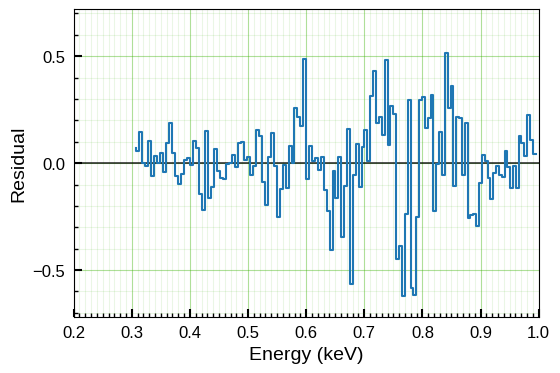
\includegraphics[width=\textwidth]{figures/resid/mr-vel-0111150101-pn_resid.png}
            \caption{Residuals between data and best-fit model for EPIC-pn observations}
            \label{fig:pn:resid}
        \end{subfigure}
        \hfill
        \begin{subfigure}[b]{0.39\textwidth}
            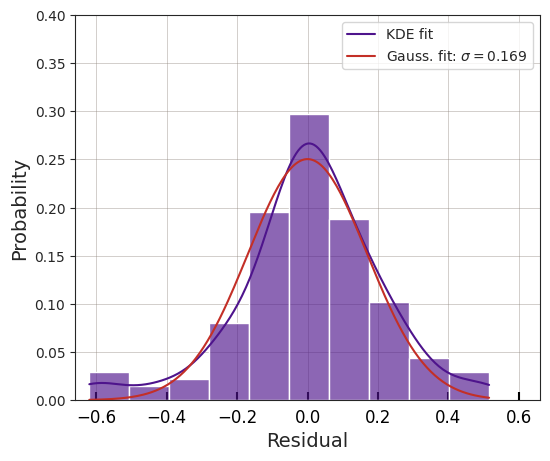
\includegraphics[width=\textwidth]{figures/resid/mr-vel-0111150101-pn_resid-hist.png}
	        \caption{Distribution of residuals from the best-fit model to EPIC-pn observations, along with the KDE function and fitted Gaussian}
	        \label{fig:pn:resid-hist}
        \end{subfigure}
        \caption{Residual statistics from best-fit model to all observations}
        \label{fig:all-obs:resid-stats}
    \end{figure*}
    
    As it can be seen in figure \ref{fig:pn:resid-hist}, the kernel density estimate (KDE) function of the distribution closely approximates a normal distribution centred about zero (with zero indicating a perfect fit) and with a standard deviation of 0.169, thereby indicating that the observed count rate data can be considered to be random fluctuations which are normally distributed about the best-fit model. Therefore, the normal distribution of the residuals indicates that they are random and do not have a systematic bias (as is expected of a good fit), thereby further validating that the model fitting performed is satisfactory for all six cases of the observations.
    
    \begin{figure}[!htb]
    	\centering
    	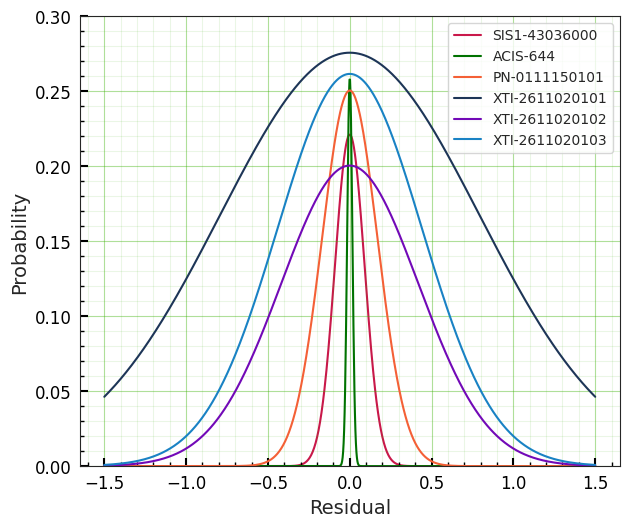
\includegraphics[width=0.45\textwidth]{figures/resid/mr-vel-resid-gaussfit_all-obs.png}
    	\caption{Gaussian approximations of the KDE functions for residual distributions of all observations}
    	\label{fig:all-obs:resid-gaussfit}
    \end{figure}
    
    In figure \ref{fig:all-obs:resid-gaussfit}, we find the Gaussian distribution fitted to all the observations. This figure shows that the quality of the fit is the best for the earlier Chandra, XMM-Newton and ASCA observations. For the recent NICER observations, the residuals show a wider spread spread about the perfect fit.
    
    %The facts that the reduced $\chi^2$ values are acceptable for a good fit and the residuals are normally distributed about zero
    
    \subsection{NLTE pure H model atmosphere}
    Rauch model atmosphere \cite{werner1999classical,rauch2003grid,rauch2010nlte}
    
%    NLTE (non-local thermal equilibrium) stellar atmosphere models
%(Werner & Dreizler 1999; Rauch 2003; Rauch & Deetjen 2003;
%Rauch et al. 2010b). Some of them are available as tables that are
%suitable for analysis within the XSPEC environment; in general,
%these models – or pre-calculated grids – differ from each other by
%the abundance of elements, by their temperature and by the effective
%gravity (expressed as log g, in cgs units). Once the specific abundance
%and gravity are chosen, the fitting to the data is parameterised by the
%effective temperature.
%Amongst the NLTE stellar atmosphere models, only
%the one with a pure hydrogen atmosphere (henceforth "pure H") and
%log g = 7 achieved a similar fit quality
%Also plotted in Figure 3 are the fit to data by two other NLTE mod-
%els: "H-Ca", that includes elements from H to Ca with abundance
%ratios as the Galactic halo and "H-Ni", with elements up to Ni and
%a particular metal enhanced abundance 14 based on nova V4743 Sgr
%(Rauch et al. 2010a,b). Even though aware that the H-Ca model
%was calculated with only approximate formulae to account for Stark
%broadening and is thus not suitable for precise spectral analysis, we
%reckon that this should not be an issue given the low energy resolu-
%tion of the spectra we are analysing. The H-Ni pre-calculated grid
%is only available for log g = 9, so we use this effective gravity for
%the H-Ca as well. While a reasonable agreement between data and
%model is obtained from bbody or pure H, neither of the two other
%NLTE models are able to fit the data, as evidenced by the residu-
%als, plotted in logarithm scale for clarity. Particularly, they notably
%underestimate the observed spectrum for energies beyond 0.45–
%0.5 keV. It can also be noticed that they demand a much larger effec-
%tive temperature – specially when compared to the pure H model –,
%likely due to the absorption caused by elements heavier than helium
%Besides previously mentioned models bbody,
%pure H and H-Ca (with halo abundances), we also show some other
%NLTE (from those publicly available) computed for different abun-
%dances: "pure He", a pure helium atmosphere model; "H-Ca", this
%time with solar abundances; and "He+CNO", a model with abundance
%ratios seen in some PG 1159 type objects (He:C:N:O = 33:50:2:15,
%e.g. Werner & Herwig 2006).
    
    \subsection{Relative strengths of absorption edges}
    Absorption edges are included in an XSPEC model using the multiplicative component named \texttt{edge}. On a continuum model, an absorption edge may be modelled as follows:
    \begin{align}
    	M(E)=\begin{cases}
    		{1;\quad E\leqslant E_\text{th}} \\
    		{\exp{\left[ -D\left(\dfrac{E}{E_\text{th}}\right)^{-3} \right]};\quad E> E_\text{th}}
    	\end{cases} \label{eqn:edge-comp}
    \end{align}
    In equation (\ref{eqn:edge-comp}), $E_\text{th}$ is the \textit{threshold energy} and $D$ is the \textit{absorption depth}. The model component is implemented with these two quantities being its parameters. The relative values of the absorption depths enables a comparison of the strengths of the absorption edges.
    
    The absorption depths calculated from the unfolded spectra, after obtaining the best fit to the model, are presented in table \ref{tab:abs-depth}. In all six observations, the same absorption edges were identified. For the observations made by ASCA, Chandra and XMM-Newton, the identified edges show the same trend with respect to the relative strengths of the absorption depths of these edges, i.e. the N $K$ absorption edge is the strongest, followed by the O $K$ edge, the Fe $L_3$ edge and the Ne $K$ edge with similar strengths.
    
    However, this is not the case for the three NICER observations, each of which show different edges to be the strongest. The reasons for such an inconsistency might range from instrumental effects (such as variations in the detector response with time, or changes in the gain calibration between observations) to issues with data reduction (such as inconsistencies in background subtraction, or inaccuracies in deadtime correction). Because NICER is a relatively new mission, it is a worthwhile exercise to investigate this particular inconsistency in absorption depth strength, which would include a detailed review of the NICER calibration documents, analysis of data from different detector regions, comparison with published data on similar sources and submission of relevant science proposals for new observations.